%===============================================================================
\chapter{Identifica��o de sistemas n�o lineares de tempo discreto}
\label{chapter:nlin_si_ident}
%===============================================================================

Anteriormente foram introduzidos conceitos b�sicos de identifica��o de sistemas lineares invariantes no tempo.
Este cap�tulo tem como objetivo apresentar os principais conceitos para identifica��o de sistemas n�o lineares de tempo
discreto.

Na Se��o \ref{sec:nlin_si_basic} ser�o apresentados conceitos b�sicos sobre n�o linearidades, algumas das principais
n�o linearidades encontradas e uma breve descri��o de suas caracter�sticas.

Na Se��o \ref{sec:nl_models} ser�o apresentados alguns modelos tipicamente utilizados para caracteriza��o de sistemas
n�o lineares. Na Se��o \ref{sec:nl_models_narmax} ser� dado �nfase aos modelos racionais e na Se��o
\ref{sec:nl_si_algorithms_rationals} ser� apresentado um algoritmo para a identifica��o de sistemas n�o lineares quando
descritos por esta estrutura de modelos. No Ap�ndice \ref{appendix:rational_base_functions} s�o apresentadas as rotinas
desenvolvidas em Matlab para o desenvolvimento deste algoritmo.

Ao fim, ser�o apresentados breves conclus�es sobre identifica��o de sistemas n�o lineares (Se��o
\ref{sec:nl_conclusions}).

%===============================================================================
%===============================================================================
\section{Conceitos b�sicos}
\label{sec:nlin_si_basic}
%===============================================================================

Muitos, se n�o todos, os sistemas reais s�o n�o lineares. Existe entretanto um grande n�mero destes sistemas que
podem, e assim o s�o, representados por sistemas lineares em determinadas faixas de opera��o. Os sistemas desta
forma conseguem representar satisfatoriamente o sistema observado. Todavia alguns sistemas para serem
linearizados exigem uma faixa de atua��o muito estreita, fazendo com que o sistema em sua opera��o normal j� saia desta
faixa, tornando o modelo linear n�o representativo para aquele sistema em quest�o.

Tem-se desta forma uma das justificativas de escolher um modelo n�o linear para caracterizar o sistema. Ganha-se de um
lado no quesito de faixa de atua��o mais ampla e perde-se por abdicar da simplicidade de sistemas lineares.

Um sistema n�o linear pode ser genericamente descrito por:

\begin{equation}
y(t)=f(u(t), e(t))
\label{eq:nlin_system}
\end{equation}
onde $f(\cdot)$ � uma fun��o n�o linear dependente do sinal de entrada $u(t)$, e do ru�do do sistema $e(t)$. $y(t)$
� definido como a sa�da deste sistema.

%===============================================================================
\subsection{Tipos de n�o linearidades}
\label{sec:nlin_si_basic_types}
%===============================================================================
% Khalil
% ljng 		142
% Aguirre

Existem duas limita��es b�sicas para sistemas linearizados. Primeiro que a lineariza��o
� uma aproxima��o ao redor do ponto de opera��o, logo ele pode prever apenas o comportamento
nesta localidade do sistema e n�o o comportamento global. Segundo, as din�micas
de sistemas n�o lineares s�o muito mais ricas que as de sistemas lineares. Existem portanto alguns
fen�menos {\it{essenciais}}, n�o lineares, que n�o conseguem ser descritos ou
preditos por modelos lineares, estes s�o: \cite{khalil}

\renewcommand{\labelitemi}{$\bullet$}
\begin{itemize}

\item Tempo de fuga finito

O estado de um sistema linear inst�vel tende ao infinito na medida que o tempo 
tende ao infinito. Um sistema n�o linear est�vel, entretanto, pode ir para o
infinito em um tempo finito.


\item M�ltiplos pontos de equil�brios isolados

Um sistema linear assintoticamente est�vel tem apenas um ponto de equil�brio. Desta forma, este sistema pode
ter apenas um ponto do espa�o de estados que atraem o estado do sistema, independentemente
do estado inicial. Um sistema n�o linear pode ter mais de um ponto de equil�brio isolado. 
Desta forma o estado do sistema pode convergir para um destes equil�brios ou outro,
dependendo do estado inicial.

\item Ciclos limites

Para um sistema linear e invariante no tempo oscilar ele deve ter um par de autovalores
sobre o eixo imagin�rio, o que � uma condi��o n�o robusta praticamente imposs�vel de manter
na presen�a de perturba��es. Mesmo que isso seja poss�vel de manter, a amplitude da 
oscila��o depender� das condi��es iniciais do sistema. Na vida real, oscila��es est�veis
s�o atingidas apenas com sistemas n�o lineares. Alguns sistemas possuem oscila��es com
amplitude e frequ�ncia constantes, independente das condi��es iniciais. Chama-se isso de
ciclos limites.

\item Sub harm�nicas, harm�nicas ou oscila��es quase peri�dicas 

Um sistema linear est�vel sob uma entrada senoidal peri�dica produz uma sa�da senoidal na mesma frequ�ncia.
Sistemas n�o lineares alimentados por sinais peri�dicos podem oscilar com frequ�ncias que
podem ser sub m�ltiplos ou m�ltiplos da frequ�ncia de entrada.

\item Caos

Um sistema n�o linear pode ter um espa�o de estados mais complexo e seu comportamento n�o 
pode ser descrito por equil�brio, oscila��es peri�dicas ou quase peri�dicas. Este comportamento
normalmente � conhecido como caos. Alguns destes movimentos ca�ticos exibem comportamento
rand�mico, independentemente da natureza do sistema.

\item M�ltiplos modos de comportamento

N�o � incomum para dois ou mais modelos exibirem o comportamentos diferentes para um mesmo sistema n�o-linear.Um sistema
n�o for�ado pode ter mais de um ciclo limite. Um sistema for�ado com excita��o pode exibir harm�nicas, sub-harm�nicas, ou
comportamentos mais complicados, dependendo da frequ�ncia e amplitude da entrada. Ele pode exibir um pulo descontinuo no
modo de comportamento mesmo com mudan�as pequenas na amplitude e frequ�ncia de entrada do sinal.

\end{itemize}




%===============================================================================
\section{Modelos para sistemas n�o lineares}
\label{sec:nl_models}
%===============================================================================
% ideia aqui � colocar uma pequena introdu��o sobre modelos.. no mesmo estilo
% que foi para sistemas lineares.

Fam�lias ou conjuntos de modelos para sistemas podem ser divididos em dois grupos principais, baseados na natureza de
suas n�o linearidades: n�o linearidades est�ticas, onde a din�mica do sistema pode ser bem caracterizada por um modelo
linear enquanto que a parte n�o linear est� concentrada ou na entrada ou na sa�da do sistema de forma est�tica.
Para estes sistemas a forma mais usual de caracterizar � utilizando a classe de modelos de Wiener para n�o linearidades
na sa�da do processo ou a classe de Hammerstein, quando a n�o linearidade est� na entrada do processo.

Para os demais casos, onde a n�o linearidade est� na din�mica do processo existem v�rias fam�lias de modelos
que podem ser utilizados como ser� visto no decorrer deste cap�tulo. De forma geral todos estes conjuntos
possuem em comum a ideia da escolha de uma base que seja representativa e que possa reduzir a quantidade de
termos a ser identificado e com isso ter uma boa aproxima��o do sistema real com a menor quantidade de
par�metros poss�vel na identifica��o.

Percebe-se ent�o que um mesmo sistema pode ser representado por diversos destes modelos, mas dependendo das
caracter�sticas deste sistema, uma das fam�lias ser� mais adequada, por sua base possuir mais
afinidade em representar certos tipos de n�o linearidades.

Um dos passos mais desafiadores na constru��o de modelos n�o lineares � a escolha da estrutura de
modelo. Quando este modelo � n�o linear, existe uma grande quantidade de op��es e com isso o perigo
de escolher um modelo desnecessariamente complexo � evidente. Isso baseia-se no {\it{principio
da parcim�nia}} que basicamente determina que o modelo deve ser o mais simples poss�vel.
\cite{aguirre_maps}

%TODO: achar onde por isso e se nao tem nada melhor no paper para adicionar
%Um problema fundamental referente a modelos parametrizados refere-se ao fato do
%par�metro poder ou n�o ser determinado a partir dos valores medidos de entrada e sa�da. \cite{glad_ljung}

% ===============================================================================
\subsection{Modelos de Wiener e Hammerstein}
\label{sec:nl_models_wiener_hammerstein}
% Aguirre: 334
% ljung 143
%===============================================================================

Modelos de Wiener e Hammerstein s�o normalmente utilizados em situa��es onde a din�mica do sistema pode ser bem
descrita por um sistema linear, mas existem algumas n�o linearidades est�ticas atreladas a entrada
e/ou a sa�da. Este ser� o caso de atuadores n�o lineares com caracter�sticas como satura��o, zona morta, entre outros.

Um modelo com n�o linearidades na entrada � chamado de {\it{modelo de Hammerstein}} e 
para n�o linearidades na sa�da chama-se {\it{modelo de Wiener}}. \cite{ljung}

Na Figura (\ref{fig:nl_models_hammerstein_wiener}) observa-se o diagrama de bloco para os modelos
de Hammerstein e Wiener.


\begin{figure}[htbp]
\center
\scalebox{1} % Change this value to rescale the drawing.
{
\begin{pspicture}(0,-1.6)(9.439062,1.6)
\usefont{T1}{ptm}{m}{n}
\rput(0.52453125,1.31){$u(t)$}
\usefont{T1}{ptm}{m}{n}
\rput(3.9557812,1.31){$f(u(t))$}
\usefont{T1}{ptm}{m}{n}
\rput(7.554531,1.35){$y(t)$}
\usefont{T1}{ptm}{m}{n}
\rput(5.8759375,1.15){Modelo}
\usefont{T1}{ptm}{m}{n}
\rput(5.7834377,0.75){Linear}
\usefont{T1}{ptm}{m}{n}
\rput(2.1957812,1.03){$f(\cdot)$}
\psframe[linewidth=0.04,dimen=outer](3.0,1.6)(1.2,0.4)
\psframe[linewidth=0.04,dimen=outer](6.8,1.6)(5.0,0.4)
\psline[linewidth=0.04cm,arrowsize=0.05291667cm 2.0,arrowlength=1.4,arrowinset=0.4]{->}(3.0,1.0)(5.0,1.0)
\psline[linewidth=0.04cm,arrowsize=0.05291667cm 2.0,arrowlength=1.4,arrowinset=0.4]{->}(0.0,1.0)(1.2,1.0)
\psline[linewidth=0.04cm,arrowsize=0.05291667cm 2.0,arrowlength=1.4,arrowinset=0.4]{->}(6.8,1.0)(8.0,1.0)
\usefont{T1}{ptm}{m}{n}
\rput(0.52453125,-0.69){$u(t)$}
\usefont{T1}{ptm}{m}{n}
\rput(3.9357812,-0.69){$z(t)$}
\usefont{T1}{ptm}{m}{n}
\rput(2.0759375,-0.85){Modelo}
\usefont{T1}{ptm}{m}{n}
\rput(1.9834375,-1.25){Linear}
\usefont{T1}{ptm}{m}{n}
\rput(5.9957814,-0.99){$f(\cdot)$}
\psframe[linewidth=0.04,dimen=outer](3.0,-0.4)(1.2,-1.6)
\psframe[linewidth=0.04,dimen=outer](6.8,-0.4)(5.0,-1.6)
\psline[linewidth=0.04cm,arrowsize=0.05291667cm 2.0,arrowlength=1.4,arrowinset=0.4]{->}(3.0,-1.0)(5.0,-1.0)
\psline[linewidth=0.04cm,arrowsize=0.05291667cm 2.0,arrowlength=1.4,arrowinset=0.4]{->}(0.0,-1.0)(1.2,-1.0)
\psline[linewidth=0.04cm,arrowsize=0.05291667cm 2.0,arrowlength=1.4,arrowinset=0.4]{->}(6.8,-1.0)(8.0,-1.0)
\usefont{T1}{ptm}{m}{n}
\rput(8.204532,-0.65){$y(t)=f(z(t))$}
\end{pspicture} 
}
\caption{Acima: modelo de Hammerstein. Abaixo: Modelo de Wiener.}
\label{fig:nl_models_hammerstein_wiener}
\end{figure}

%===============================================================================
\subsection{Serie de volterra}
\label{sec:nl_models_volterra}
% Aguirre 334
%===============================================================================

Um sistema n�o linear pode ser descrito pela serie de Volterra \eqref{eq:nl_models_volterra}:

\begin{equation}
y(t)=\sum_{j=1}^{\infty}\int_{-\infty}^{\infty}\cdots \int_{-\infty}^{\infty}
h_j(\tau_1, ... ,\tau_j) \prod_{i=1}^{j}u(t-\tau_i)d\tau_i
\label{eq:nl_models_volterra}
\end{equation}

Onde $h_j$ s�o generaliza��es n�o lineares da resposta ao impulso $h_1(t)$ . Para
um sistema linear com $j=1$ a equa��o de Volterra se reduz a integral de convolu��o.
\cite{aguirre}

As expans�es funcionais em series de Volterra relacionam os sinais passados da entrada com o valor atual da sa�da do
sistema e isso inevitavelmente significa que que um conjunto excessivo de par�metros � necess�rio para descrever at� mesmo
simples sistemas n�o lineares e consequentemente apenas poucas aplica��es pr�ticas foram apresentadas.
\cite{chen_billings1989}

%===============================================================================
\subsection{Redes Neurais}
\label{sec:nl_models_neurals}
% TODO: Search for bib
%===============================================================================
As redes neurais artificiais s�o compostas por camadas de neur�nios interconectados. A sa�da de um
neur�nio com $n$ entradas � apresentado na equa��o \eqref{eq:nl_models_neural}

\begin{equation}
x=\emph{f}\left ( \sum_{j=1}^{n}\omega_j x_j +b \right )
\label{eq:nl_models_neural}
\end{equation}

Sendo $b$ (bias) e $\omega_j$ constantes. $\emph{f}(\cdot)$ � chamada fun��o de ativa��o. A
fun��o de ativa��o mais comum �: \cite{aguirre}

\begin{equation}
\emph{f}(z)=\frac{1}{1+e^{-z}}
\nonumber
\end{equation}


%===============================================================================
\subsubsection{Redes Neurais multi-camadas}
\label{sec:nl_models_neurals_multilayer}
%===============================================================================

Uma tipica rede multi-camadas pode ser descrita como na Figura
(\ref{fig:nl_models_neural_multilayer}).  Na pratica redes neurais multi-camadas tem grande apelo no
reconhecimento de padr�es. Do ponto de vista te�rico os sistemas de redes multi-camadas podem ser
considerados como mapas n�o lineares onde os elementos das matrizes de peso s�o os par�metros.
\cite{narenda_parthasarathy}

\begin{figure}[htbp]
\center
\scalebox{0.85} % Change this value to rescale the drawing.
{
\begin{pspicture}(0,-3.369375)(14.589063,3.329375)
\pscircle[linewidth=0.04,dimen=outer](4.77,2.729375){0.4}
\usefont{T1}{ptm}{m}{n}
\rput(4.804531,2.699375){$\sum$}
\psframe[linewidth=0.04,dimen=outer](7.17,3.329375)(5.97,2.129375)
\usefont{T1}{ptm}{m}{n}
\rput(6.534531,2.759375){$\gamma$}
\pscircle[linewidth=0.04,dimen=outer](4.77,0.529375){0.4}
\usefont{T1}{ptm}{m}{n}
\rput(4.804531,0.499375){$\sum$}
\psframe[linewidth=0.04,dimen=outer](7.17,1.129375)(5.97,-0.070625)
\usefont{T1}{ptm}{m}{n}
\rput(6.534531,0.559375){$\gamma$}
\pscircle[linewidth=0.04,dimen=outer](4.77,-1.870625){0.4}
\usefont{T1}{ptm}{m}{n}
\rput(4.804531,-1.900625){$\sum$}
\psframe[linewidth=0.04,dimen=outer](7.17,-1.270625)(5.97,-2.470625)
\usefont{T1}{ptm}{m}{n}
\rput(6.534531,-1.840625){$\gamma$}
\pscircle[linewidth=0.04,dimen=outer](10.37,2.729375){0.4}
\usefont{T1}{ptm}{m}{n}
\rput(10.384531,2.679375){$\sum$}
\psframe[linewidth=0.04,dimen=outer](12.77,3.329375)(11.57,2.129375)
\usefont{T1}{ptm}{m}{n}
\rput(12.254531,2.739375){$\gamma$}
\pscircle[linewidth=0.04,dimen=outer](10.37,0.529375){0.4}
\usefont{T1}{ptm}{m}{n}
\rput(10.384531,0.479375){$\sum$}
\psframe[linewidth=0.04,dimen=outer](12.77,1.129375)(11.57,-0.070625)
\usefont{T1}{ptm}{m}{n}
\rput(12.254531,0.539375){$\gamma$}
\pscircle[linewidth=0.04,dimen=outer](10.37,-1.870625){0.4}
\usefont{T1}{ptm}{m}{n}
\rput(10.384531,-1.920625){$\sum$}
\psframe[linewidth=0.04,dimen=outer](12.77,-1.270625)(11.57,-2.470625)
\usefont{T1}{ptm}{m}{n}
\rput(12.254531,-1.860625){$\gamma$}
\psline[linewidth=0.04cm,arrowsize=0.05291667cm 2.0,arrowlength=1.4,arrowinset=0.4]{->}(5.17,2.729375)(5.97,2.729375)
\psline[linewidth=0.04cm,arrowsize=0.05291667cm 2.0,arrowlength=1.4,arrowinset=0.4]{->}(5.17,0.529375)(5.97,0.529375)
\psline[linewidth=0.04cm,arrowsize=0.05291667cm 2.0,arrowlength=1.4,arrowinset=0.4]{->}(5.37,-1.870625)(5.97,-1.870625)
\psline[linewidth=0.04cm,arrowsize=0.05291667cm 2.0,arrowlength=1.4,arrowinset=0.4]{->}(10.77,2.729375)(11.57,2.729375)
\psline[linewidth=0.04cm,arrowsize=0.05291667cm 2.0,arrowlength=1.4,arrowinset=0.4]{->}(10.77,0.529375)(11.57,0.529375)
\psline[linewidth=0.04cm,arrowsize=0.05291667cm 2.0,arrowlength=1.4,arrowinset=0.4]{->}(10.77,-1.870625)(11.57,-1.870625)
\psline[linewidth=0.04cm,arrowsize=0.05291667cm 2.0,arrowlength=1.4,arrowinset=0.4]{->}(12.77,2.729375)(13.97,2.729375)
\psline[linewidth=0.04cm,arrowsize=0.05291667cm 2.0,arrowlength=1.4,arrowinset=0.4]{->}(12.77,0.529375)(13.97,0.529375)
\psline[linewidth=0.04cm,arrowsize=0.05291667cm 2.0,arrowlength=1.4,arrowinset=0.4]{->}(12.77,-1.870625)(13.97,-1.870625)
\usefont{T1}{ptm}{m}{n}
\rput(13.674531,3.039375){$y_1$}
\usefont{T1}{ptm}{m}{n}
\rput(13.674531,0.839375){$y_2$}
\usefont{T1}{ptm}{m}{n}
\rput(13.674531,-1.560625){$y_n$}
\psdots[dotsize=0.12](6.77,-0.470625)
\psdots[dotsize=0.12](6.77,-0.670625)
\psdots[dotsize=0.12](6.77,-0.870625)
\psdots[dotsize=0.12](12.37,-0.470625)
\psdots[dotsize=0.12](12.37,-0.670625)
\psdots[dotsize=0.12](12.37,-0.870625)
\psline[linewidth=0.04cm,arrowsize=0.05291667cm 2.0,arrowlength=1.4,arrowinset=0.4]{->}(7.1873198,2.729375)(9.97,2.729375)
\psline[linewidth=0.04cm,arrowsize=0.05291667cm 2.0,arrowlength=1.4,arrowinset=0.4]{->}(7.1873198,2.729375)(9.97,0.529375)
\psline[linewidth=0.04cm,arrowsize=0.05291667cm 2.0,arrowlength=1.4,arrowinset=0.4]{->}(7.1873198,2.729375)(9.97,-1.870625)
\psline[linewidth=0.04cm,arrowsize=0.05291667cm 2.0,arrowlength=1.4,arrowinset=0.4]{->}(7.1873198,0.529375)(9.97,0.529375)
\psline[linewidth=0.04cm,arrowsize=0.05291667cm 2.0,arrowlength=1.4,arrowinset=0.4]{->}(7.1873198,-1.870625)(9.97,-1.870625)
\psline[linewidth=0.04cm,arrowsize=0.05291667cm 2.0,arrowlength=1.4,arrowinset=0.4]{->}(7.1873198,0.529375)(9.97,2.729375)
\psline[linewidth=0.04cm,arrowsize=0.05291667cm 2.0,arrowlength=1.4,arrowinset=0.4]{->}(7.1873198,0.529375)(9.97,-1.870625)
\psline[linewidth=0.04cm,arrowsize=0.05291667cm 2.0,arrowlength=1.4,arrowinset=0.4]{->}(7.1873198,-1.870625)(9.97,0.529375)
\psline[linewidth=0.04cm,arrowsize=0.05291667cm 2.0,arrowlength=1.4,arrowinset=0.4]{->}(7.1873198,-1.870625)(9.97,2.729375)
\psline[linewidth=0.04cm,arrowsize=0.05291667cm 2.0,arrowlength=1.4,arrowinset=0.4]{->}(1.7888126,2.7075653)(4.37,2.7075653)
\psline[linewidth=0.04cm,arrowsize=0.05291667cm 2.0,arrowlength=1.4,arrowinset=0.4]{->}(1.7888126,2.7075653)(4.37,0.51799595)
\psline[linewidth=0.04cm,arrowsize=0.05291667cm 2.0,arrowlength=1.4,arrowinset=0.4]{->}(1.7888126,2.7075653)(4.37,-1.870625)
\psline[linewidth=0.04cm,arrowsize=0.05291667cm 2.0,arrowlength=1.4,arrowinset=0.4]{->}(1.7871279,0.529375)(4.37,0.529375)
\psline[linewidth=0.04cm,arrowsize=0.05291667cm 2.0,arrowlength=1.4,arrowinset=0.4]{->}(1.7871279,-1.850625)(4.37,-1.850625)
\psline[linewidth=0.04cm,arrowsize=0.05291667cm 2.0,arrowlength=1.4,arrowinset=0.4]{->}(1.7871279,0.529375)(4.37,2.729375)
\psline[linewidth=0.04cm,arrowsize=0.05291667cm 2.0,arrowlength=1.4,arrowinset=0.4]{->}(1.7871279,0.529375)(4.37,-1.870625)
\psline[linewidth=0.04cm,arrowsize=0.05291667cm 2.0,arrowlength=1.4,arrowinset=0.4]{->}(1.7871279,-1.850625)(4.37,0.5389402)
\psline[linewidth=0.04cm,arrowsize=0.05291667cm 2.0,arrowlength=1.4,arrowinset=0.4]{->}(1.7871279,-1.850625)(4.37,2.729375)
\usefont{T1}{ptm}{m}{n}
\rput(1.4745313,3.039375){$u_1$}
\usefont{T1}{ptm}{m}{n}
\rput(1.4745313,0.839375){$u_2$}
\usefont{T1}{ptm}{m}{n}
\rput(1.4745313,-1.560625){$u_n$}
\usefont{T1}{ptm}{m}{n}
\rput(1.4845313,-3.160625){$\text{Entrada}$}
\usefont{T1}{ptm}{m}{n}
\rput(6.7345314,-3.160625){$\text{Camada Oculta}$}
\usefont{T1}{ptm}{m}{n}
\rput(12.444531,-3.160625){$\text{Camada Sa�da}$}
\end{pspicture} 
}

\caption{Rede neural multi-camadas.}
\label{fig:nl_models_neural_multilayer}
\end{figure}

A sa�da do sistema para uma rede multi-camadas pode ser descrito como em
\eqref{eq:nl_models_neural_multilayer}.

\begin{equation}
y(t)=f_s\left \{ \sum_{i=1}^{m} \omega_i f_i \left ( \sum_{j=1}^{n}\omega_{ij} x_j + b_i \right ) +
b_s \right \}
\label{eq:nl_models_neural_multilayer}
\end{equation}

Sendo que $f_s$ � a fun��o de ativa��o do neur�nio da camada de sa�da. Esta fun��o n�o precisa ser
igual a $f_i$, $i=1, \ldots , m$ que por sua vez n�o precisam ser iguais entre si. $b_s$ � o termo
de polariza��o do neur�nio da camada de sa�da, $\omega_i$ s�o os pesos da sa�da de cada neur�nio da
camada oculta e $\omega_{ij}$ s�o os pesos da entrada $j$, vista pelo $i-$�simo neur�nio da camada
oculta. \cite{aguirre}

%===============================================================================
\subsubsection{Redes Neurais recorrentes}
\label{sec:nl_models_neurals_multilayer}
%===============================================================================

Redes neurais recorrentes, trabalho introduzido por Hopfield em \cite{hopfield} prov� uma
alternativa para o reconhecimento de padr�es. O m�todo proposto consiste em ter uma rede neural de
apenas uma camada adicionada de uma realimenta��o com um atraso de tempo como apresentado na Figura
(\ref{fig:nl_models_neural_recurrent}). \cite{narenda_parthasarathy}

\begin{figure}[htbp]
\center
\scalebox{0.85} % Change this value to rescale the drawing.
{
\begin{pspicture}(0,-5.4)(11.04,5.4)
\usefont{T1}{ptm}{m}{n}
\rput(8.015624,4.91){$\gamma$}
\usefont{T1}{ptm}{m}{n}
\rput(8.015624,3.31){$\gamma$}
\usefont{T1}{ptm}{m}{n}
\rput(8.215624,0.71){$\gamma$}
\usefont{T1}{ptm}{m}{n}
\rput(5.073437,-0.89){$z^{-1}$}
\pscircle[linewidth=0.04,dimen=outer](6.42,4.8){0.4}
\pscircle[linewidth=0.04,dimen=outer](6.42,0.6){0.4}
\pscircle[linewidth=0.04,dimen=outer](6.42,3.2){0.4}
\usefont{T1}{ptm}{m}{n}
\rput(6.395625,0.61){$\sum$}
\usefont{T1}{ptm}{m}{n}
\rput(6.395625,3.21){$\sum$}
\usefont{T1}{ptm}{m}{n}
\rput(6.395625,4.81){$\sum$}
\psdots[dotsize=0.12](5.82,4.8)
\psdots[dotsize=0.12](5.82,3.2)
\psdots[dotsize=0.12](5.82,0.6)
\psdots[dotsize=0.12](2.82,4.8)
\psdots[dotsize=0.12](2.82,3.2)
\psdots[dotsize=0.12](2.82,0.6)
\psline[linewidth=0.04cm](2.82,4.8)(5.82,4.8)
\psline[linewidth=0.04cm](2.82,4.8)(5.82,3.1916058)
\psline[linewidth=0.04cm](2.82,4.8)(5.82,0.61817497)
\psline[linewidth=0.04cm](2.82,0.61817497)(5.82,4.8)
\psline[linewidth=0.04cm](2.82,3.1916058)(5.82,4.8)
\psline[linewidth=0.04cm](2.82,3.1916058)(5.82,3.1916058)
\psline[linewidth=0.04cm](2.82,3.1916058)(5.82,0.61817497)
\psline[linewidth=0.04cm](2.82,0.61817497)(5.82,3.1916058)
\psline[linewidth=0.04cm](2.82,0.61817497)(5.82,0.61817497)
\psline[linewidth=0.04cm](8.8,0.6)(9.42,0.6)
\psline[linewidth=0.04cm](9.4,-1.0)(5.8,-1.0)
\psline[linewidth=0.04cm](4.62,-1.0)(1.6,-1.0)
\psline[linewidth=0.04cm](1.62,0.6)(2.82,0.6)
\psline[linewidth=0.04cm](6.82,0.6)(7.62,0.6)
\psline[linewidth=0.04cm](5.82,0.6)(6.0,0.6)
\psline[linewidth=0.04cm](6.82,3.2)(7.62,3.2)
\psline[linewidth=0.04cm](5.82,3.2)(6.02,3.2)
\psline[linewidth=0.04cm](5.82,4.8)(6.02,4.8)
\psline[linewidth=0.04cm](6.82,4.8)(7.62,4.8)
\psline[linewidth=0.04cm](8.8,3.2)(10.22,3.2)
\psline[linewidth=0.04cm](5.8,-2.6)(10.2,-2.6)
\psline[linewidth=0.04cm](8.8,4.8)(11.02,4.8)
\psline[linewidth=0.04cm](11.0,-4.8)(5.8,-4.8)
\psline[linewidth=0.04cm](4.62,-2.6)(0.8,-2.6)
\psline[linewidth=0.04cm](0.8,3.2)(2.82,3.2)
\psline[linewidth=0.04cm](2.82,4.8)(0.0,4.8)
\psline[linewidth=0.04cm](0.0,-4.8)(4.62,-4.8)
\psdots[dotsize=0.12](8.22,2.2)
\psdots[dotsize=0.12](8.22,2.0)
\psdots[dotsize=0.12](8.22,1.8)
\psdots[dotsize=0.12](5.22,-3.4)
\psdots[dotsize=0.12](5.22,-3.6)
\psdots[dotsize=0.12](5.22,-3.8)
\usefont{T1}{ptm}{m}{n}
\rput(9.864062,5.11){$x_1(t+1)$}
\usefont{T1}{ptm}{m}{n}
\rput(9.864062,3.51){$x_2(t+1)$}
\usefont{T1}{ptm}{m}{n}
\rput(9.864062,0.91){$x_n(t+1)$}
\usefont{T1}{ptm}{m}{n}
\rput(2.0040624,5.11){$x_1(t)$}
\usefont{T1}{ptm}{m}{n}
\rput(2.0040624,3.51){$x_2(t)$}
\usefont{T1}{ptm}{m}{n}
\rput(2.0040624,0.91){$x_n(t)$}
\usefont{T1}{ptm}{m}{n}
\rput(4.3840623,5.11){$\omega_i$}
\usefont{T1}{ptm}{m}{n}
\rput(5.073437,-2.49){$z^{-1}$}
\usefont{T1}{ptm}{m}{n}
\rput(5.073437,-4.69){$z^{-1}$}
\psframe[linewidth=0.04,dimen=outer](8.8,5.4)(7.6,4.2)
\psframe[linewidth=0.04,dimen=outer](8.8,3.8)(7.6,2.6)
\psframe[linewidth=0.04,dimen=outer](8.8,1.2)(7.6,0.0)
\psframe[linewidth=0.04,dimen=outer](5.8,-0.4)(4.6,-1.6)
\psframe[linewidth=0.04,dimen=outer](5.8,-2.0)(4.6,-3.2)
\psframe[linewidth=0.04,dimen=outer](5.8,-4.2)(4.6,-5.4)
\psline[linewidth=0.04cm](11.0,4.8)(11.0,-4.8)
\psline[linewidth=0.04cm](10.2,3.2)(10.2,-2.6)
\psline[linewidth=0.04cm](9.4,0.6)(9.4,-1.0)
\psline[linewidth=0.04cm](1.6,0.6)(1.6,-1.0)
\psline[linewidth=0.04cm](0.8,-2.6)(0.8,3.2)
\psline[linewidth=0.04cm](0.0,4.8)(0.0,-4.8)
\end{pspicture} 
}
\caption{Rede neural recorrentes.}
\label{fig:nl_models_neural_recurrent}
\end{figure}

%===============================================================================
\subsection{Fun��es Radiais de Base}
\label{sec:nl_models_radiais}
% Aguirre 337
%===============================================================================

Fun��es radiais de base  ({\it{RBF - Radial basis functions}})  s�o uma tradicional t�cnica para
interpola��o em espa�os multidimensional \cite{chen_billings_narmax} e podem ser descritos como
mapeamentos do tipo:

\begin{equation}
f(y)=w_0+\sum_{i}w_i \phi (\left \| y-c_i \right \|)
\label{eq:nl_models_rbf}
\end{equation}

Sendo que $y \in \mathbb{R}^{d_e}$ ($d_e$ � conhecido como dimens�o de imers�o),
$\left \| \cdot \right \|$ � a norma euclidiana, $w_i \in \mathbb{R}$ s�o pesos, 
$c_i \in \mathbb{R}^{d_e}$ s�o centros e $\phi(\cdot):\mathbb{R}^+ \to \mathbb{R}$ 
� uma fun��o, normalmente escolhida a priori, como por exemplo: \cite{aguirre}

\begin{equation}
\phi(\left \| y-c_i \right \|)= exp\left ( -\frac{\left \| y-c_i \right \|^2}{\sigma_i^2} \right )
\nonumber
\end{equation}

Outras fun��es de base usadas s�o apresentadas na Tabela \ref{table:nl_models_rbf}

\begin{table*}[htbp]
\begin{center}
\caption{Algumas fun��es Radiais de base comumente utilizadas.}
\label{table:nl_models_rbf}
\begin{tabular}{ll}
\hline
        Nome & Fun��o   \\
\hline
        Multi quadr�tica inversa  & $\phi(r)=(r^2+\sigma ^2)^{-1/2}$ \\ 
        Linear                    & $\phi(r)=r$                      \\ 
        C�bica                    & $\phi(r)=r^3$                    \\ 
        Multi-quadr�tica           & $\phi(r)=\sqrt{r^2+\sigma^2}$    \\ 
        {\it{Thin - plate spline}} & $\phi(r)=r^2\; \text{log}(r)$   \\ 
\hline
\end{tabular}
\end{center}
\end{table*}

Sendo que $r=\left \| y-c_i \right \|$ e $\sigma$ definem a largura do chap�u no caso de
fun��es Gausianas e das multi-quadr�ticas, como pode ser visto na figura (\ref{fig:nl_models_rbf}).

\begin{figure}[htbp]
	\center
	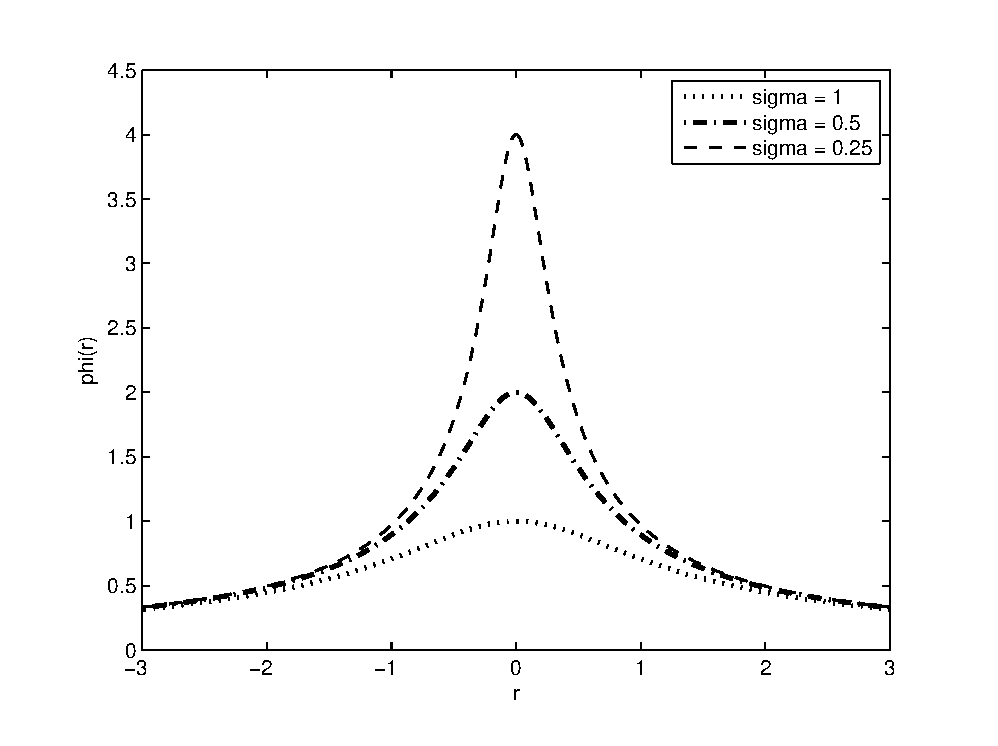
\includegraphics[width=0.8\columnwidth]{figures/nl_models_rbf.eps}
	\caption{Fun��o multiquadr�ticas inversa para alguns valores de $\sigma$.}
	\label{fig:nl_models_rbf}
\end{figure}

Este tipo de representa��o tem boas propriedades locais e pode ser interpretada como 
uma t�cnica de interpola��o global. Fun��es radiais de base s�o casos particulares
de redes neurais, porem neste caso lineares nos par�metros $w_i$.\cite{aguirre} 

No contexto de identifica��o de sistemas � comum adicionar termos auto-regressivos
lineares, bem como termos de entrada � equa��o \eqref{eq:nl_models_rbf} resultando em:

\begin{equation}
y(k)=w_0 + \sum_{i}w_i \phi(\left \| \mathbf{y}(k-1)-c_i \right \|)+\sum_{i=1}^{n_y}a_i y(k-i)+\sum_{i=1}^{n_u}b_i u(k-i)+e(k)
\nonumber
\end{equation}

Sendo $\mathbf{y}(k-1)=\begin{bmatrix}
y(k-1) & ... & y(k-n_y) & u(k-1) & ... & u(k-n_u)
\end{bmatrix}$.

%===============================================================================
\section{Algoritmo para identifica��o de modelos racionais}
\label{sec:nl_si_algorithms_rationals}
%===============================================================================

Esta se��o descreve um algoritmo para determinar os par�metros de modelos racionais
do tipo apresentado em \eqref{eq:nl_model_narmax_rat_simp}. Este algoritmo foi proposto por
\cite{correa} e � uma modifica��o do algoritmo originalmente proposto por
\cite{billings_zhu}. Assume-se que o modelo pode ser aproximado por: \cite{aguirre}

\begin{eqnarray}\nonumber
y(t)&=&\frac
{a(y(t-1), ..., y(t-n_y), u(t-1), ..., u(t-n_u))}
{b(y(t-1), ..., y(t-n_y), u(t-1), ..., u(t-n_u))}\\
&&  +c(e(t-1), ... , e(t-n_e)) +e(t)
\label{eq:nl_alg_rational}
\end{eqnarray}

Onde o ru�do � modelado por um polin�mio que pode ou n�o ser linear. A considera��o b�sica 
por tr�s de \eqref{eq:nl_alg_rational} � que o erro de regress�o pode ser representado por
um modelo {\it{MA}}({\it{Move average}}), possivelmente n�o linear. Assim sendo sugere-se o 
seguinte procedimento: \cite{aguirre}

\begin{enumerate}

%==========================================================================
% Step 1
\item Fa�a $i=0$. Monte a matriz $\Psi$ de regress�o e estime os coeficiente usando
o m�todo dos m�nimos quadrados:

\begin{equation}
\begin{bmatrix}
\hat{\theta}_n^i\\ 
\hat{\theta}_{d1}^i
\end{bmatrix}=\left [ \Psi ^T \Psi \right ]^{-1}\Psi^T y^*
\label{nl_alg_rational_step_1}
\end{equation}

onde o �ndice $i$ indica a itera��o. Al�m disso a matriz de regressores $\Psi$ � 
formada tomando-se os vetores de regressores $\psi_n(t-1)$ e $\psi_{d1}(t-1)$ ao longo
da janela de dados do tamanho $N$, ou seja:

\begin{equation}
\Psi=\begin{bmatrix}
\psi_n^T(t-1) & \psi_{d1}^T(t-1)\\ 
\vdots & \vdots \\ 
\psi_n^T(t+N-2) & \psi_{d1}^T(t+N-2)
\end{bmatrix}
\nonumber
\end{equation}

Analogamente o vetor $y^* \in \mathbb{R} ^{N \times 1}$ � formado tomando os dados,
ou seja:

\begin{equation}
y^{*T}=\left [ y^*(t), y^*(t+1), ..., y^*(t+N-1) \right ]
\nonumber
\end{equation}

%==========================================================================
% Step 2
\item Fa�a $i=i+1$. Determine os res�duos e sua vari�ncia, respectivamente como:

\begin{equation}
\xi ^i(t)=y(t)-\frac{\psi_n^T(t-1)\hat{\theta}_n}{\psi_{d}^T(t-1)\hat{\theta}_d}
\label{nl_alg_rational_step2_res}
\end{equation}

\begin{equation}
\left ( \sigma _{\xi}^2 \right )^i=\frac{1}{N-m_d}\sum_{i=m_d+1}^{N}\left ( \xi ^i(t) \right )^2
\label{eq:nl_alg_rational_step2_var}
\end{equation}

onde $N$ � o tamanho dos dados e $m_d=max(n_y, n_u, n_e)$.

%==========================================================================
% Step 3
\item Usando-se os res�duos determinados no passo anterior, atualize $\Psi ^T \Psi$ e $\Psi^T y^*$
usando:

\begin{equation}
\Psi=\begin{bmatrix}
\psi_{n}^T(t-1) & y(t)\psi_{d1}^T(t-1)  & \psi_{\xi }^T(t-1) \\ 
\vdots & \vdots & \vdots\\ 
\psi_{n}^T(t+N-2) & y(t)\psi_{d1}^T(t+N-2)  & \psi_{\xi }^T(t+N-2)
\end{bmatrix}
\label{eq:nl_alg_rational_step3_psi}
\end{equation}

onde $\psi_{\xi }$ � o vetor de regressores do modelo do ru�do. Pelo fato do ru�do n�o ser medido,
os res�duos do passo (2) s�o utilizados.

%==========================================================================
% Step 4
\item Determine

\begin{equation}
\Phi =\begin{bmatrix}
0      & \dots & 0      & 0 & \dots & 0 & \dots & 0 & \dots & 0\\ 
\vdots &       & \vdots & \vdots &  & \vdots &  & \vdots &  & \vdots\\ 
0      & \dots & 0      & \sum_{t=1}^{N}p_{d2}^2 & \dots & \sum_{t=1}^{N}p_{d2}p_{d_{N_d}}  & \dots & 0 & \dots & 0\\ 
\vdots &       & \vdots & \vdots &  & \vdots &  & \vdots &  & \vdots\\ 
0      & \dots & 0      & \sum_{t=1}^{N}p_{dN_d}p_{d2} & \dots & \sum_{t=1}^{N}p_{d_{N_d}}^2 & \dots & 0 & \dots & 0 
\end{bmatrix}
\label{eq:nl_alg_rational_step5_Psi}
\end{equation}

\begin{equation}
\phi =\begin{bmatrix}
0\\ 
\vdots\\ 
0\\ 
-\sum_{k=1}^{N} p_{d2}p_{d1}\\ 
\vdots\\ 
-\sum_{k=1}^{N} p_{dN_d}p_{d1}\\ 
0\\ 
\vdots\\
0
\end{bmatrix}
\label{eq:nl_alg_rational_step5_phi}
\end{equation}


E estime novamente os par�metros utilizando:

\begin{equation}
\begin{bmatrix}
\hat{\theta}_n^i\\ 
\hat{\theta}_{d1}^i
\end{bmatrix}=\left [ \Psi^T \Psi - (\sigma _{\xi}^2)^i \Phi  \right ]^{-1}
\left [ \Psi^T y^* - (\sigma _{\xi}^2)^i \phi \right ]
\label{eq:nl_alg_rational_step5}
\end{equation}

%==========================================================================
% Step 5
\item Volte ao passo 2 at� atingir converg�ncia (de par�metro ou de vari�ncia de res�duo).
\end{enumerate} % Aguirre algorithm for rational model identification pg 394


A converg�ncia do algoritmo depende da converg�ncia da estimativa da sequ�ncia do ru�do.
\cite{billings_zhu91} 

%===============================================================================
\subsection{Exemplos ilustrativos}
\label{sec:nl_si_algorithms_rationals_examples}
%===============================================================================

Nesta se��o ser�o apresentados alguns casos de uso do algoritmo descrito anteriormente. 
Inicia-se com um exemplo simples, onde o sistema � racional e a classe de modelos escolhida consegue representar
completamente este sistema ($\mathcal{S} \in \mathcal{M}$). Em seguida ser� apresentado um exemplo onde o sistema ainda
� racional, mas a classe de modelos escolhida n�o consegue representar completamente o sistema em quest�o, ou seja,
$\mathcal{S} \notin \mathcal{M}$. Por fim ser� apresentado um exemplo real de um conversor de corrente cont�nua para
corrente cont�nua do tipo Buck.

Ser�o apresentados os resultados obtidos a fim de verificar a qualidade e a confiabilidade do algoritmo de identifica��o
de sistemas NARMAX, polinomial e racional.

%===============================================================================
\subsubsection{Sistemas originalmente racionais}
\label{sec:nl_si_algorithms_rationals_ex1}
%===============================================================================

Considere o sistema real:

\begin{equation}
y(t)=\frac{0.2 y(t-1)+0.1 y(t-1)u(t-1)+ u(t-1)}{1+y^{2}(t-1)+y^{2}(t-2)}+e(t)
\label{eq:nl_rat_exemple2}
\end{equation}

O modelo escolhido para representar o sistema real �:

\begin{equation}
y(t)=\frac{\theta_1 y(t-1)+\theta_2 y(t-1)u(t-1)+ \theta_3u(t-1)}{1+\theta_4 y^{2}(t-1)+ \theta_5y^{2}(t-2)}
\label{eq:nl_rat_exemple2_model}
\end{equation}

Utilizando para simula��o um sinal PRBS de 635 pontos e adicionando-se um ru�do $e(t)$ de vari�ncia $\sigma_e^2=0.005$
os resultados da m�dia de 100 estimativas de Monte Carlo foram:

\begin{equation}
\theta_{\text{m�dia}} =\begin{bmatrix}
0.1991  &  0.0995  &  0.9963  &  0.9899  &  0.9912
\end{bmatrix}
\nonumber
\end{equation}

%A vari�ncia encontrada foi de:
%
%\begin{equation}
%\theta_{\text{vari�ncia}} =1.0\times 10^{-4} \begin{bmatrix}
%0.0089  &  0.0073  &  0.1082  &  0.7179  &  0.7910
%\end{bmatrix}
%\nonumber
%\end{equation}

A matriz de covari�ncia encontrada:

\begin{equation}
\theta_{\text{Covari�ncia}} =1.0\times 10^{-4} \begin{bmatrix}
    0.0089 & -0.0005 & 0.0112 & 0.0213 & 0.0339 \\
   -0.0005 &  0.0073 & 0.0057 & 0.0220 & 0.0091 \\
    0.0112 &  0.0057 & 0.1082 & 0.2529 & 0.2589 \\
    0.0213 &  0.0220 & 0.2529 & 0.7179 & 0.4987 \\
    0.0339 &  0.0091 & 0.2589 & 0.4987 & 0.7910
\end{bmatrix}
\nonumber
\end{equation}

Utilizando a m�dia das estimativas para simular a sa�da do modelo obtido com o sistema real, obteve-se um
custo:

\begin{equation}
V(\theta)=1.1269\times 10^{-4}
\nonumber
\end{equation}

A fim de melhor ilustrar a estimativa obtida, na Figura \ref{fig:nl_rat_example2} s�o apresentadas as
estimativas dos par�metros $\theta_1$ e $\theta_2$ e a elipse de confian�a para $\chi^2=95\%$.

\begin{figure}[htbp]
	\center
	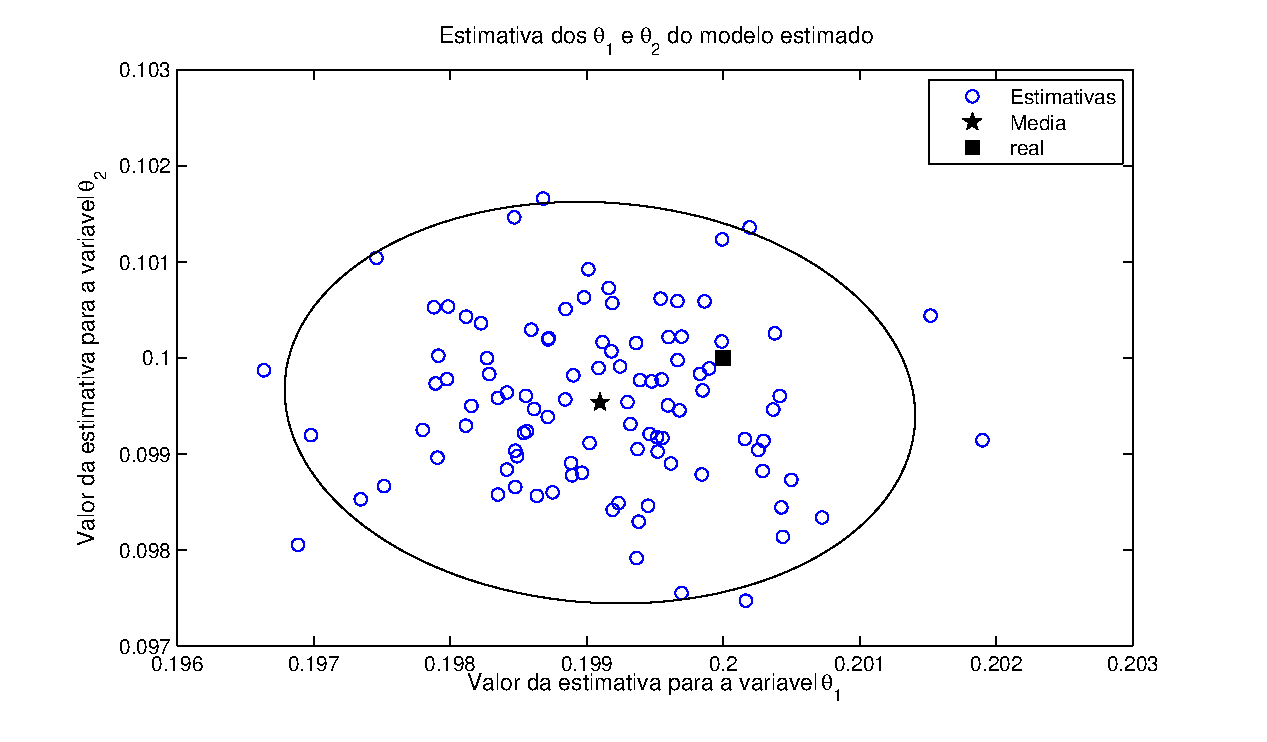
\includegraphics[width=0.9\columnwidth]{figures/rat_example2_a1_a2.eps}
	\caption{Estimativas obtidas nos 100 experimentos de Monte Carlo realizados para as vari�veis $\theta_1$ e
	$\theta_2$.}
	\label{fig:nl_rat_example2}
\end{figure}

Devido a presen�a de ru�do e ao erro de polariza��o apresentado ser menor que a vari�ncia do ru�do adicionado, sabe-se
que com o aumento de $N$ o valor de $\hat{\theta}_N \to \theta_0$.

%===============================================================================
\subsubsection{Sistemas originalmente racionais, quando $\mathcal{S} \notin \mathcal{M}$}
\label{sec:nl_si_algorithms_rationals_ex2}
%===============================================================================

Considere o sistema real:

\begin{equation}
y(t)=\frac{0.2 y(t-1)+0.1 y(t-1)u(t-1)+u(t-1)}{1+y^{2}(t-1)+y^{2}(t-2)}
\label{eq:nl_rat_exemple3}
\end{equation}

O sistema real $\mathcal{S}$ n�o consegue ser representada pela classe de modelos escolhida:

\begin{equation}
y(t)=\frac{\theta_1y(t-1)+\theta_2u(t-1)}{1+\theta_3y^{2}(t-1)+\theta_4y^{2}(t-2)}
\label{eq:nl_rat_exemple3_model}
\end{equation}

Utilizando par a simula��o um sinal PRBS de 635 pontos e um ru�do de vari�ncia $\sigma_e^2=0.005$ os resultados
da m�dia de 100 estimativas de Monte Carlo foram:

\begin{equation}
\theta_{\text{m�dia}} =\begin{bmatrix}
0.2279  &  1.1341  &  1.2716  &  1.3769
\end{bmatrix}
\nonumber
\end{equation}

%A vari�ncia encontrada foi de:
%
%\begin{equation}
%\theta_{\text{vari�ncia}} =1.0\times 10^{-3} \begin{bmatrix}
%0.0020  &  0.0535  &  0.3402  &	  0.3217
%\end{bmatrix}
%\nonumber
%\end{equation}

A fim de comparar a qualidade dos resultados obtidos, na Figura \ref{fig:nl_rat_example3} � apresentadas a resposta do
sistema real \eqref{eq:nl_rat_exemple3} e o sistema obtido pela estimativa utilizando o a classe de modelos
\eqref{eq:nl_rat_exemple3_model} para uma entrada do tipo degrau unit�rio.

\begin{figure}[htbp]
	\center
	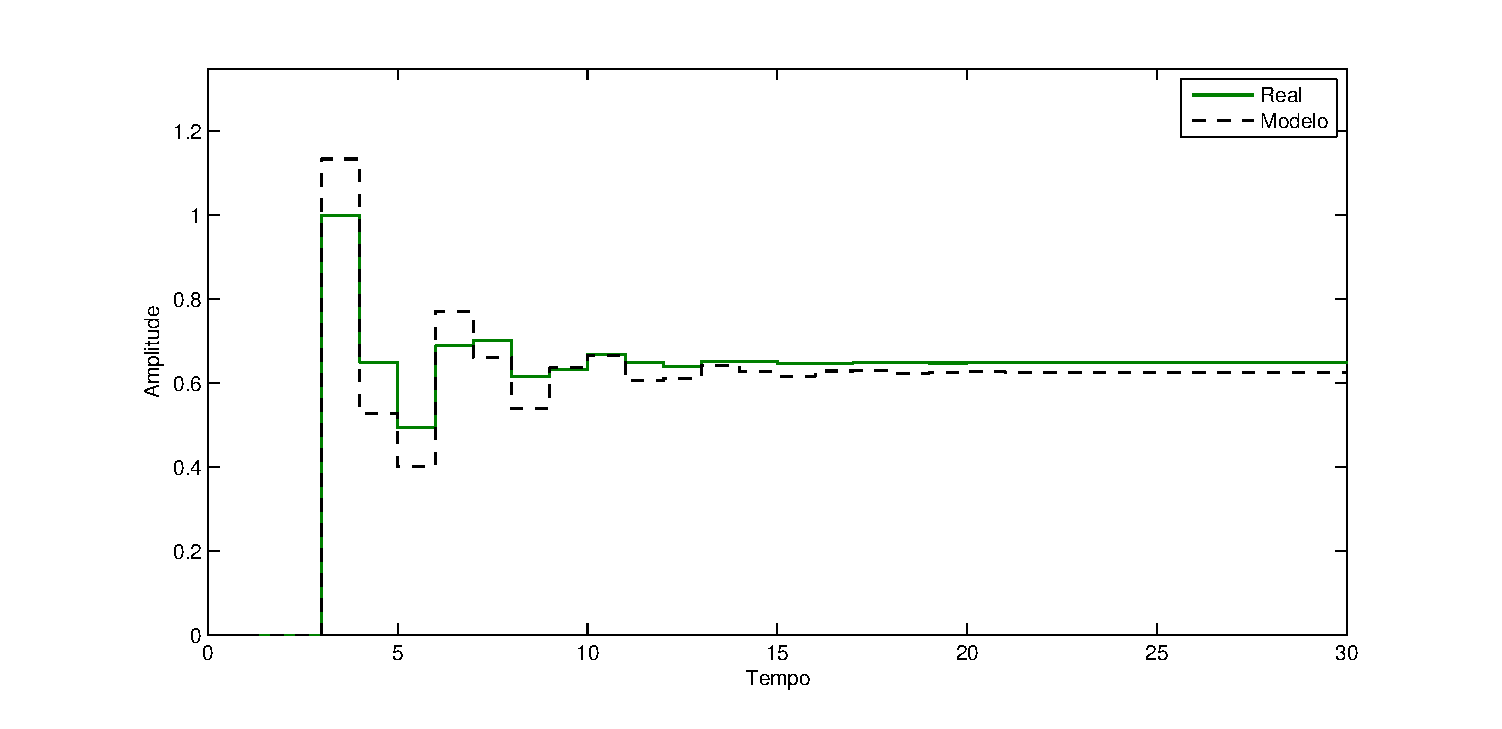
\includegraphics[width=0.9\columnwidth]{figures/rat_example3.eps}
	\caption{Exemplo 2 - Comparativo da resposta do sistema real e do modelo estimado para uma entrada do tipo degrau
	unit�rio}
	\label{fig:nl_rat_example3}
\end{figure}

O custo obtido para o modelo estimado foi de:

\begin{equation}
V(\theta)=1.1239
\nonumber
\end{equation}

Como n�o h� um valor de $\theta_0$ para compara��o, visto que o sistema real n�o consegue ser presentado pelo modelo,
optou-se por apresentar o resultado do sistema a uma resposta do tipo degrau unit�rio. Observa-se com isso que o sistema
estimado � apenas semelhante ao real, possuindo um sobrepasso maior e possuindo um ganho em regime ligeiramente
diferente que o sistema real. 
%===============================================================================
\subsubsection{Conversor CC-CC Buck}
\label{sec:nl_si_algorithms_rationals_buck}
% Aguirre 397
% Tese do corr�a - pg 27
%===============================================================================
O conversor de corrente cont�nua do tipo Buck possui um mapa n�o linear que pode ser obtido a partir da equa��o do
circuito apresentado na Figura \ref{fig:nl_models_buck_circuit} e que tem a forma como em: \cite{tse_buck}

\begin{equation}
y(t)=\alpha y(t-1)+\frac{h(d_n)^2 \beta E\left [ E-y(t-1) \right ]}{y(t-1)}
\label{eq:nl_alg_buck_circ}
\end{equation}
onde $\alpha = 0.8872$, $\beta = 1.2$ e $E=33$ s�o constantes que dependem apenas dos componentes do
circuito eletr�nico. $d_n$ � um sinal de tens�o que implementa a a��o de controle e a satura��o
$h(d_n)$ � dada por :

\begin{equation}
h(d_n)=\left\{\begin{matrix}
0 & \text{se } d_n < 0\\ 
1 & \text{se } d_n > 1\\ 
d_n & \text{caso contrario.}
\end{matrix}\right.
\nonumber
\end{equation}

\begin{figure}[htbp]
	\center
	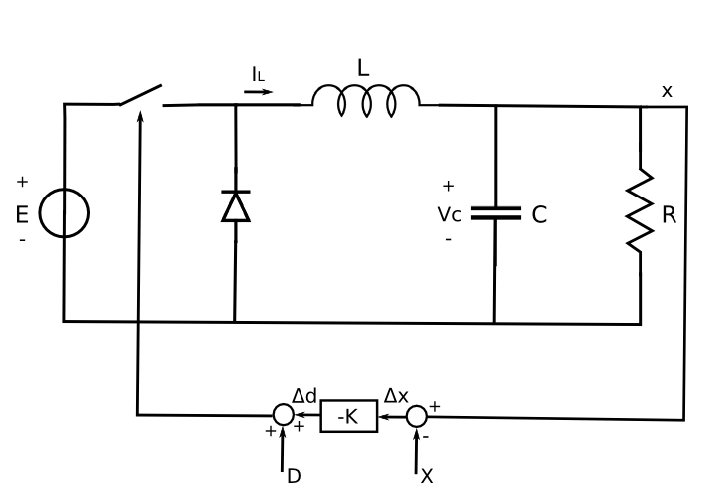
\includegraphics[width=0.55\columnwidth]{figures/nl_models_buck_circuit.eps}
	\caption{Circuito do conversor CC-CC Buck}
	\label{fig:nl_models_buck_circuit}
\end{figure}

Modelos polinomiais n�o resultam em bons modelos para a din�mica de \eqref{eq:nl_alg_buck_circ}. Um
modelo com estrutura {\it{ad rock}}, que aproxima relativamente bem a caracter�stica est�tica do
conversor �: \cite{aguirre_maps}

\begin{equation}
y(t)=O exp\left [ 22-y(t-1) \right ]+ \frac{a\; y(t-1)^2 -b\; y(t-1)+c}{y(t-1)}
\nonumber
\end{equation}
onde $O=46.429$, $a=2.6204$, $b=99.875$ e $c=1.4171\times 10^3$. Por outro lado a 

Para aplicar o algoritmo, escolhe-se inicialmente um modelo para o sistema em an�lise. O modelo
racional

\begin{equation}
y(t)=\frac{8.658+0.1223\times10^{-2}y(t-1)^3-0.441\times10^{-1}y(t-1)^2}
{1-0.8381\times10^{-1}y(t-1)+0.1766\times10^{-2}y(t-1)^2}
\label{eq:nl_alg_buck_rational}
\end{equation}
aproxima bem a din�mica em quest�o. \cite{aguirre}

Para a utiliza��o do algoritmo, escolheu-se um modelo com a forma:

\begin{equation}
y(t)=\frac{\theta_1+\theta_2y(t-1)^3+\theta_3(t-1)^2}{1+\theta_4y(t-1)+\theta_5y(t-1)^2}
\label{eq:nl_alg_buck_rational_model}
\end{equation}

Os par�metros da equa��o \eqref{eq:nl_alg_buck_rational} s�o os valores de refer�ncia para a utiliza��o do
m�todos descrito em \cite{aguirre}. Utilizando o algoritmo previamente apresentado, o resultado da estimativa
foi:

\begin{equation}
\theta =\begin{bmatrix}
8.8807 & 8.6698\times 10^{-4} &-0.0359 &-0.0736 & 0.0013 
\end{bmatrix}
\nonumber
\end{equation}

Como pode ser observado, pelos resultados de $\theta$ obtidos e os valores esperados, existe polariza��o na
estimativa obtida. Isso em parte se d� pela falta de capacidade da classe de modelos escolhida em representar
o processo real e pela escolha do modelo de ru�do que para este caso foi apenas utilizado o erro da
estimativa, com rela��o a sa�da do sistema real obtido.

Foram utilizadas amostras de 100 pontos para esta estimativa e realizados 100 experimentos de Monte Carlo.
Os resultados obtidos foram de uma m�dia de:

\begin{equation}
\text{m�dia de }\;\theta =\begin{bmatrix}
8.8976  &    8.6762\times 10^{-4}    & -0.0360 &  -0.0736  &  0.0013
\end{bmatrix}
\nonumber
\end{equation}

com uma covari�ncia de 

\begin{equation}
\theta_{\text{Covari�ncia}} = 1.0\times 10^{-3}\begin{bmatrix}
 0.4842 &  0.0000 & -0.0011 &  0.0007 &-0.0000 \\
 0.0000 &  0.0000 & -0.0000 & -0.0000 & 0.0000 \\
-0.0011 & -0.0000 &  0.0000 & -0.0000 & 0.0000 \\
 0.0007 & -0.0000 & -0.0000 &  0.0000 &-0.0000 \\
-0.0000 &  0.0000 &  0.0000 & -0.0000 & 0.0000 
\end{bmatrix}
\nonumber
\end{equation}


%===============================================================================
\section{Considera��es Finais}
\label{sec:nl_conclusions}
%===============================================================================


%===============================================================================

